\documentclass[UTF8]{ctexart}
\usepackage{listings}
\usepackage{booktabs}  
\usepackage{geometry}  
\usepackage{graphicx} 
\usepackage{xcolor}
\usepackage{float}
\usepackage{array}
\usepackage{enumitem}
\usepackage{amsmath,amssymb,bm}
\usepackage[version=4]{mhchem}
\usepackage{siunitx}
\usepackage{tikz}
\usepackage{pgfplots}
\pgfplotsset{compat=1.18}
% 移除biblatex,使用natbib进行引用管理
\usepackage[numbers,sort&compress]{natbib}
\usepackage[colorlinks=true]{hyperref} 
\usepackage{xurl} 
\usepackage{url}
\hypersetup{
    colorlinks = true,
    linkcolor = blue,
    citecolor = blue,
    urlcolor = blue,
    pdftitle = {CFD Final Project},
    pdfsubject = {Computational Fluid Dynamics},
    pdfauthor = {朱林}
}

\pgfplotsset{compat=1.18}
\graphicspath{{figure/}}
\geometry{a4paper, left=2.5cm, right=2.5cm, top=2.5cm, bottom=2.5cm}
\definecolor{codegreen}{rgb}{0,0.6,0}
\definecolor{codegray}{rgb}{0.5,0.5,0.5}
\definecolor{codepurple}{rgb}{0.58,0,0.82}
\lstset{
    basicstyle=\ttfamily\footnotesize,
    breaklines=true,
    frame=single,
    numbers=left,
    numberstyle=\tiny\color{codegray},
    keywordstyle=\color{blue},
    commentstyle=\color{codegreen},
    stringstyle=\color{codepurple},
    showstringspaces=false
}



\begin{document}
\title{计算流体力学期末大作业}
\author{朱林-2200011028}
\date{\today}
\maketitle

\section{数理算法原理}
\subsection{问题描述}
\subsubsection{物理情形}
Sod激波管问题是一个一维理想气体流动问题:无限长管道中,初始时刻($t=0$)在$x=0$处有一薄膜分隔两侧气体:
\begin{itemize}
    \item 左侧($x<0$): 高压区,状态为$(\rho_L, u_L, p_L)$
    \item 右侧($x>0$): 低压区,状态为$(\rho_R, u_R, p_R)$
\end{itemize}

薄膜在$t=0^+$时刻瞬时破裂,两侧气体开始相互作用,产生复杂的波系结构。

\subsubsection{标准初始条件}
采用以下无量纲初始条件:
\begin{align*}
\text{左侧:} & \quad \rho_L = 1.0,  u_L = 0.0,  p_L = 1.0 \\
\text{右侧:} & \quad \rho_R = 0.125,  u_R = 0.0,  p_R = 0.1
\end{align*}

\subsection{控制方程}
流动由一维欧拉方程描述:
\begin{align}
&\frac{\partial \mathbf{U}}{\partial t} + \frac{\partial f(\mathbf{U})}{\partial x} = 0 \\
&\mathbf{U} = \begin{bmatrix} \rho \\ \rho u \\ E \end{bmatrix}, \quad
f(\mathbf{U}) = \begin{bmatrix} \rho u \\ \rho u^2 + p \\ u(E + p) \end{bmatrix}
\end{align}
其中总能密度$E = \rho e = \rho (C_v T + \frac{1}{2}u^2)$。

\subsection{Riemann问题精确解}
\subsubsection{波系结构}
根据空气动力学知识,该 Sod 激波管中可能出现三种波:
\begin{itemize}
    \item 激波:流体密度、速度、压力均发生突变,满足 Rankine-Hugoniot (R-H) 关系式。
    \item 接触间断:流体仅密度发生突变,速度与压力不变。
    \item 膨胀波(稀疏波):一种等熵波,其内部物理量连续、光滑,头、尾物理量连续但导数不连续(弱间断),且 Riemann 不变量不变。
\end{itemize}
对于一维sod激波管问题,薄膜破裂后将形成向左传播的膨胀波、向右传播的接触间断和激波,如图\ref{fig:wave_structure_1}。
这些波将流场划分为五个特征区域(如图\ref{fig:wave_structure_2}所示\footnote{url:https://blog.csdn.net/Nidebear/article/details/109300513}):
\begin{figure}[H]
    \centering
    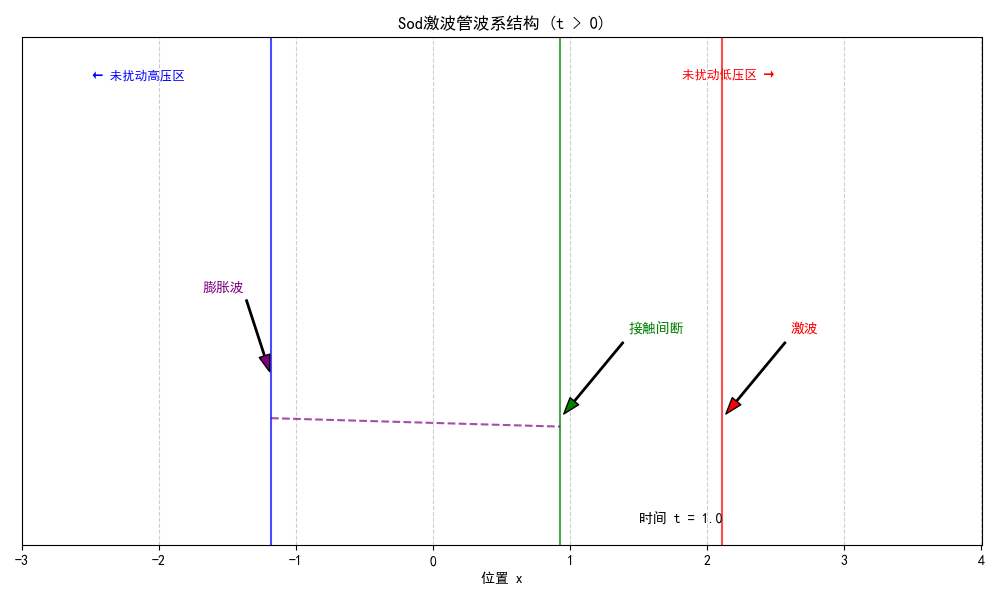
\includegraphics[width=0.8\textwidth]{wave_structure_1.png}
    \caption{Sod激波管典型波系结构(t>0)}
    \label{fig:wave_structure_1}
\end{figure}
\begin{figure}[H]
    \centering
    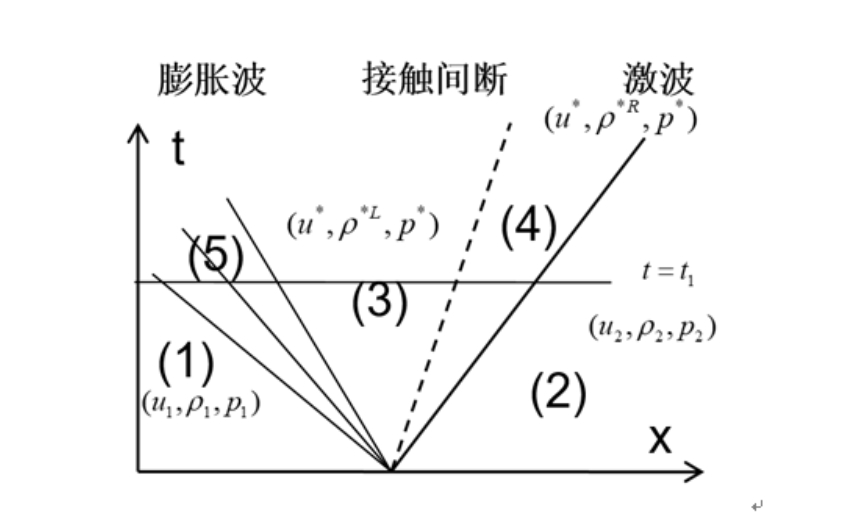
\includegraphics[width=0.8\textwidth]{wave_structure_2.png}
    \caption{Sod激波管典型波系结构}
    \label{fig:wave_structure_2}
\end{figure}
\begin{itemize}
    \item \textbf{区域1} 未扰动的左侧高压区,保持初始状态 $(\rho_L, u_L, p_L)$
    \item \textbf{区域2} 未扰动的右侧低压区,保持初始状态 $(\rho_R, u_R, p_R)$
    \item \textbf{区域3} 膨胀波后,状态为 $(\rho_2, u^*, p^*)$
    \item \textbf{区域4} 接触间断与激波间均匀区,状态为 $(\rho_3, u^*, p^*)$
    \item \textbf{区域5} 膨胀波内部
\end{itemize}

其中 $u^*$ 和 $p^*$ 为接触间断处的速度和压力,各波位置随时间线性变化:
$$x_{\text{left}} = -c_L t, \quad x_{\text{contact}} = u^* t, \quad x_{\text{shock}} = W_s t$$
$W_s$ 为激波传播速度,$c_L = \sqrt{\gamma p_L/\rho_L}$ 为左侧声速。

\subsubsection{解析解表达式}
解析解通过求解以下方程组获得:
\paragraph{1-3 两区, 等熵关系式}
\begin{equation}
    \frac{p^{*}}{\left(\rho^{* L}\right)^{\gamma}}=\frac{p_{1}}{\left(\rho_{1}\right)^{\gamma}}
\end{equation}
\begin{equation}
u_{1}+\frac{2 c_{1}}{\gamma-1}=u^{*}+\frac{2 c^{L}}{\gamma-1}
\end{equation}
其中, $c^{L}=\sqrt{\gamma p^{*} / \rho^{* L}}$。
\paragraph{2-4 两区, 激波 R-H 关系式}
\begin{equation}
\left\{\begin{array}{l}\rho_{2}\left(u_{2}-Z_{2}\right)=\rho^{* R}\left(u^{*}-Z_{2}\right) \\\rho_{2} u_{2}\left(u_{2}-Z_{2}\right)+p_{2}=\rho^{* R} u^{*}\left(u^{*}-Z_{2}\right)+p^{*} \\E_{2}\left(u_{2}-Z_{2}\right)+u_{2} p_{2}=E^{* R}\left(u^{*}-Z_{2}\right)+p^{*} u^{*}\end{array}\right.
\end{equation}
以上变量说明从略。综上 5 个方程、 5 个未知数,故方程组可解,求解方法为联立以上两个方程组,解出 3、4 区内速度对压力的依赖关系,有

$$u^{*}=u_{1}-f(p^{*},p_{1},\rho_{1})$$

其中,满足 
\begin{equation}
f(p^{*},p_{i},\rho_{i})=\frac{2c_{i}}{\gamma-1}\left[\left(\frac{p^{*}}{p_{i}}\right)^{\frac{\gamma-1}{2\gamma}}-1\right]
\end{equation}
注意到,激波、膨胀波前后速度-压力的依赖关系可写成统一的形式:

左波(激波或膨胀波)

$$u^{*}=u_{1}-f(p^{*},p_{1},\rho_{1})$$

右波(激波或膨胀波)

$$u^{*}=u_{2}+f(p^{*},p_{2},\rho_{2})$$

以上 $u^{*},p^{*}$ 表示 3、4 区内的速度与压力,其中

\begin{equation}
f(p^{*},p_{i},\rho_{i})=\left\{\begin{array}{ll}\frac{p^{*}-p_{i}}{\rho_{i}c_{i}\left[\frac{\gamma+1}{2\gamma}\left(\frac{p^{*}}{p_{i}}\right)+\frac{\gamma-1}{2\gamma}\right]^{1/2}}, & p^{*}>p_{i}\\\frac{2c_{i}}{\gamma-1}\left[\left(\frac{p^{*}}{p_{i}}\right)^{\frac{\gamma-1}{2\gamma}}-1\right], & p^{*}<p_{i}\end{array}\right.
\end{equation}

求解上式可得到 3、4 区内的压力,然后可以解得速度和密度。
\paragraph{膨胀波内部}

对于膨胀波内部物理量的计算,首先由波头传播速度$u_1-c_1$与波尾传播速度$u^*-c^{*L}$
可计算膨胀波的范围。在膨胀波区内,利用特征相容关系和等熵关系计算物理量,可利
用简单波的特性来简化计算。以下直接给出各个物理量的计算表达式:
$$\begin{aligned}&c(t,x)=\frac{\gamma-1}{\gamma+1}\left(u_{1}-\frac{x}{t}\right)+\frac{2}{\gamma+1}c_{1}\\&u(x,t)=c+x/t\\&p=p_{1}\:(c/c_{1})^{2\gamma/\gamma-1}\\&\rho=\gamma p/c^{2}\end{aligned}$$
综上所述,一维 Riemann 问题的精确解的求解思路与方程介绍完毕。本文 Sod 激波管参考
精确解程序来自于 GitLab 上的项目 simple shock tube calculator \cite{sodcal2025}。

\subsection{数值计算方法}
% 补充边界条件说明
\subsubsection{计算域与网格}

计算域设置为 $x \in [-5, 5]$,时间计算域为 $t \in [0, 2.0]$,该范围足以捕捉Sod问题中激波、接触间断和膨胀波的完整演化过程。空间离散采用均匀网格划分,网格间距 $\Delta x$ 由计算域长度和网格数动态确定。时间步长 $\Delta t$ 根据CFL条件自适应调整:

\begin{equation}
\Delta t = \text{CFL} \cdot \frac{\Delta x}{\max(|u| + c)}
\end{equation}

边界条件采用无反射处理:
\begin{align*}
U_0 &= U_1 \\
U_{N+1} &= U_N
\end{align*}
此边界处理可有效抑制数值反射,确保波系在计算域内自由传播。网格收敛性研究表明,接触间断分辨率对网格依赖性显著,需足够细密的网格才能准确捕捉密度突变特征。

\subsubsection{激波捕捉格式}
\paragraph{1. TVD格式:}
TVD(总变差递减)格式通过限制器函数控制空间离散的振荡特性,其核心原理为:
\begin{equation}
\phi(r) = \max[0, \min(1,r)] \quad (r=\text{梯度比})
\end{equation}
采用MUSCL(单调上游中心格式)重构框架,通过斜率限制实现:
1. 单元界面状态线性重构:$U_{i+1/2} = U_i + \frac{\phi}{2}\Delta U$
2. 通量计算采用Riemann求解器
3. 时间推进使用三阶Runge-Kutta
该格式在激波附近自动降阶,保持单调性但引入数值耗散,对接触间断分辨率有限。

\paragraph{2. 群速度控制:}
群速度控制(GVC)格式通过修正通量抑制高频振荡,其物理基础为:
\begin{equation}
F^{\text{GVC}} = (1-\alpha)F^{\text{high}} + \alpha F^{\text{low}}
\end{equation}
核心计算步骤:
1. 计算特征速度$\lambda_k$及其空间梯度
2. 构建控制因子$\alpha$,正比于特征速度变化率
3. 混合高精度通量与低耗散通量
当检测到特征速度剧烈变化(激波区域)时,自动增强耗散项抑制非物理振荡,光滑区域保持高阶精度。

\paragraph{3. WENO格式:}
加权本质无振荡(WENO)格式采用自适应模板选择策略:
\begin{equation}
F_{i+1/2} = \sum_{k} \omega_k F_k
\end{equation}
数值实现要点:
1. 构建多个候选插值模板(左偏、中心、右偏)
2. 计算各模板光滑指示器$\beta_k$:$\beta_k \propto \sum (\Delta^l U)^2$
3. 设计非线性权重$\omega_k \sim 1/(\beta_k + \epsilon)^p$
4. 加权组合各模板通量
该格式在间断附近自动选择最光滑模板,保持高阶精度的同时实现本质无振荡,对膨胀波分辨率尤为优越。


\subsubsection{数值通量计算方法}
\paragraph{1. FVS (通量矢量分裂)}
通量矢量分裂的核心思想是将Euler通量分解为正向传播和逆向传播分量:
\begin{equation}
f(U) = f^+(U) + f^-(U)
\end{equation}
计算原理:
1. 基于局部特征速度进行通量分裂:
\begin{equation}
f^{\pm} = \frac{1}{2}(f(U) \pm \alpha U)
\end{equation}
其中$\alpha$为最大特征速度
2. Steger-Warming分裂方案:
\begin{equation}
f^{\pm} = \frac{1}{2}\left(\rho u \pm \rho |u|\right) + \cdots
\end{equation}
3. 界面通量计算:
\begin{equation}
f_{i+1/2} = f^+(U_L) + f^-(U_R)
\end{equation}
该格式结构简单但引入数值耗散,特别适合激波捕捉,但接触间断分辨率有限。

\paragraph{2. FDS (通量差分裂)}
通量差分裂方法基于Riemann问题精确解思想:
\begin{equation}
f_{i+1/2} = \frac{1}{2}\left[f(U_L) + f(U_R)\right] - \frac{1}{2}\sum_{k=1}^{3} \alpha_k |\lambda_k| r_k
\end{equation}
计算步骤:
1. 计算界面左右状态$U_L, U_R$
2. 构造Jacobian矩阵$A = \partial f/\partial U$
3. 特征分解:$A = R\Lambda L$
4. 计算波强度$\alpha = L \cdot (U_R - U_L)$
5. 组装通量:
\begin{equation}
f_{i+1/2} = \frac{1}{2}[f(U_L) + f(U_R)] - \frac{1}{2}R|\Lambda|L \Delta U
\end{equation}
Roe格式作为典型FDS方法,在光滑区域保持高精度,但需熵修正避免激波后振荡。

\subsubsection{时间推进格式}
采用三阶Runge-Kutta方法离散时间项,其Butcher表为:
\begin{center}
\begin{tabular}{c|ccc}
0 & & & \\
1/2 & 1/2 & & \\
1 & -1 & 2 & \\
\hline
& 1/6 & 2/3 & 1/6
\end{tabular}
\end{center}
计算流程:
\begin{align}
U^{(1)} &= U^n + \Delta t \mathcal{L}(U^n) \\
U^{(2)} &= \frac{3}{4}U^n + \frac{1}{4}U^{(1)} + \frac{1}{4}\Delta t \mathcal{L}(U^{(1)}) \\
U^{n+1} &= \frac{1}{3}U^n + \frac{2}{3}U^{(2)} + \frac{2}{3}\Delta t \mathcal{L}(U^{(2)})
\end{align}
其中$\mathcal{L}(U)$为空间离散算子。此格式具有:
1. 三阶时间精度
2. 强稳定性保持(SSP)特性
3. 大时间步长稳定性
4. 与高精度空间格式良好兼容

\subsubsection{附加题:特征重构方法在FVS框架中的应用}
\label{sec:char_recon}

特征重构方法的核心思想是将守恒变量投影到特征空间进行处理,其数学基础为:
\begin{equation}
W = L \cdot U, \quad L = \text{左特征矩阵}
\end{equation}

在FVS框架中的实施步骤:\\
1. \textbf{局部特征分解}:
   \begin{equation}
   A = \frac{\partial f}{\partial U} = R\Lambda L
   \end{equation}
   其中$\Lambda = \text{diag}(\lambda_k)$为特征值矩阵

2. \textbf{特征变量投影}:
   \begin{equation}
   W_L = L \cdot U_L, \quad W_R = L \cdot U_R
   \end{equation}

3. \textbf{特征空间重构}:
   \begin{align}
   W_{i+1/2}^L &= \text{Recon}(W_{i-1}, W_i, W_{i+1}) \\
   W_{i+1/2}^R &= \text{Recon}(W_i, W_{i+1}, W_{i+2})
   \end{align}
   采用WENO/TVD等重构技术

4. \textbf{物理空间恢复}:
   \begin{equation}
   U_{i+1/2}^L = R \cdot W_{i+1/2}^L, \quad U_{i+1/2}^R = R \cdot W_{i+1/2}^R
   \end{equation}

5. \textbf{FVS通量计算}:
   \begin{equation}
   f_{i+1/2} = f^+(U_{i+1/2}^L) + f^-(U_{i+1/2}^R)
   \end{equation}



%附录
\newpage
\appendix
\section*{AI工具使用声明表}
\begin{table}[H]
    \centering
    \begin{tabular}{c|c|c}
        \hline
        使用内容 & 工具名称 & 使用目的 \\ \hline
        hw2.tex 1-9行、图片插入 & Github Copilot & 调整pdf格式,调用宏包,省略插入图片的重复性工作 \\ 
        main.py 6-15行 & DeepSeek & 修正 matplotlib 中文显示问题 \\ 
        ReadMe.md框架 & DeepSeek & 在DeepSeek的帮助下生成一个框架,在此基础上增加而来 \\
        .gitignore & Github Copilot & 针对于python和latex的.gitignore文件,完全由Copilot生成  
    \end{tabular}
    \label{tab:AI_tools}
\end{table}


\newpage
\section*{}
% 使用标准的BibTeX格式
\bibliographystyle{unsrturl} % 更改为支持URL的样式
\bibliography{reference} % 指定BibTeX数据库文件

\end{document}